\documentclass[11pt]{article}
%\usepackage{abbrevs}
\usepackage{natbib}
\usepackage{hyperref}
\usepackage{graphicx}     % could insert ``draft'' between []
\usepackage{caption}
\usepackage{subcaption}
\pagestyle{empty}

\setlength{\oddsidemargin}{0pt} % there is 1 inch before the
                                % side margin in ``article'' class
\setlength{\textwidth}{6.5in}

\setlength{\voffset}{0pt}
%\setlength{\topmargin}{-36pt}     % there is 1 inch before the
\setlength{\topmargin}{-0.75in}     % there is 1 inch before the
                                % top margin in ``article'' class and
                                % then room for header, etc.
\setlength{\textheight}{9.5in}
%%%%%%%%%%%

\begin{document}
{\centering{\bf\Large HERA:  Discussion Design} \\}
{
\centering{\bf\large Hydrogen Epoch of Reionization Array \\}
}
\vspace*{0.5cm}

%\tableofcontents
%\newpage

\section{Introduction}

The Hydrogen Epoch of Reionization Array (HERA) project 

This document provide an initial discussion design (aka strawman).  It is meant
to introduce one plausible system design for discussion.  The design is then to
be iterated to the point of a first version of a real architecture and design.
Figure \ref{fig:overall} shows an overall block diagram of the system,
identifying the major subsystems, which are discussed below.  Note that blocks
bordered with dashed lines indicate optional or variational elements.

The design is for about 1000 elements.  As discussed below, the elements will
likely be aggregated in groups of three at the node and groups of eight in the
digital system, so the target number is 3 $\times$ 8 $\times$ 42 = 1008
elements.

\begin{figure}[h]
\centering
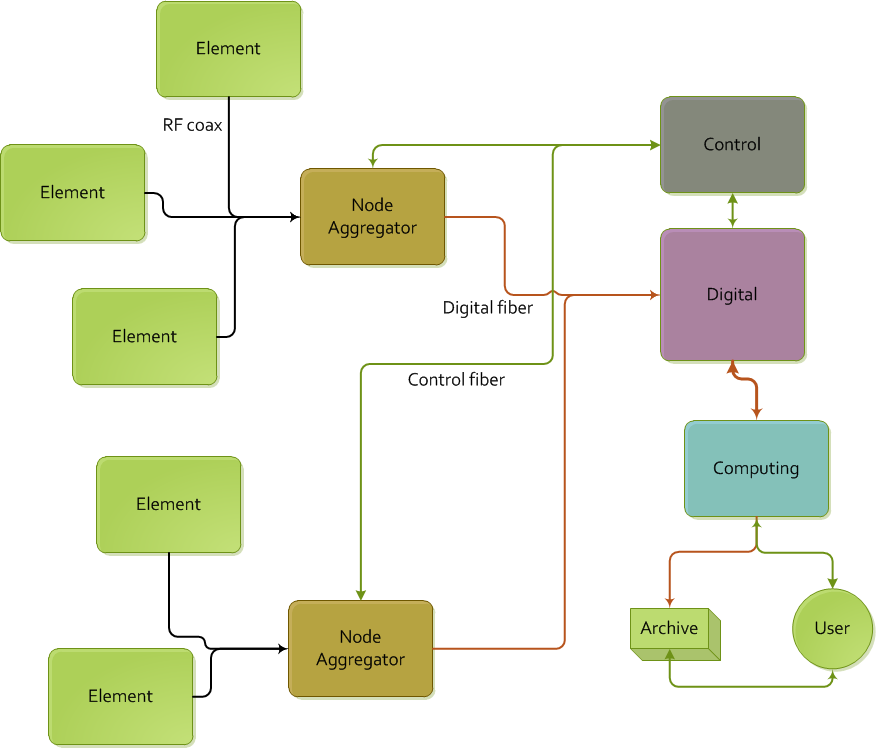
\includegraphics[width=0.75\textwidth]{plots/Overall.png}
\caption{Overall system block diagram.}
\label{fig:overall}
\end{figure}

\section{Element}

The Element sub-system is meant to maximize the sensitivity with minimal
hardware.  The sub-system consists of identical elements that are aggregated at
a node.  The connection between the two has the following interfaces:

\begin{itemize}
\item Two RF cables (50 $\Omega$, Type-N)
\item DC power (2-conductor \#18)
\item Ground (1-conductor \#18)
\item Control (2-conductor \#24)
\end{itemize}

Figure \ref{fig:elements} shows two possible layouts of dipoles as well as
indicating the accompanying RF hardware possibilities.  An optional phase
switch is shown, which may also go at the node or be omitted.  It is not
desired to have at the element since logic or faster switching signals are then
needed at that location, however it has the greatest potential performance at
that location.

\begin{figure}
\begin{subfigure}[h]{0.5\textwidth}
\centering
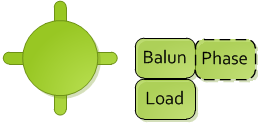
\includegraphics[width=\textwidth]{plots/Element1.png}
\caption{Single-dipole element.}
\label{fig:element1}
\end{subfigure}
\begin{subfigure}{0.5\textwidth}
\centering
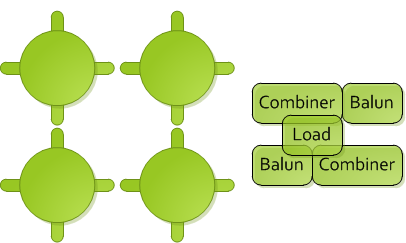
\includegraphics[width=\textwidth]{plots/Element4.png}
\caption{Four-dipole element.}
\label{fig:element4}
\end{subfigure}
\caption{Element configurations.}
\label{fig:elements}
\end{figure}

Other elements shown there are the balun/amplifier and a load switch, which
would be controlled by the two control conductors.  This allows a calibration
resistor to be switched in and out.

In order to maximize sensitivity for a given size correlator, the dipoles may
be combined in a static, zenith beamformer (combiner).  Depending on the
performance details, the combiner may precede the balun to limit hardware
needed.

\section{Node}

The concept of the node which aggregates elements is important for a
hierarchical, extensible system that is desired and is diagrammed in Figure
\ref{fig:node}.  The node accepts the RF signals and supplies power and any
needed (limited) control to the elements.  The node digitizes the signals and
sends them back on aggregated optical fibers to the digital system.  A key
desireable feature is for the node to derive its own synchronized clock using a
GPS-based system.  Additionally a locally-based small solar power system that
could power it and the associated antennas would make a truly extensible and
flexible system.

\begin{figure}[h]
\centering
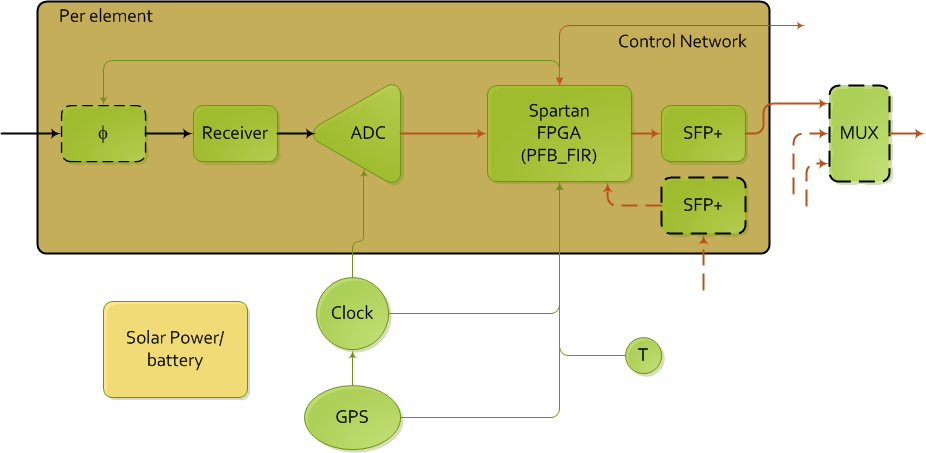
\includegraphics[width=0.85\textwidth]{plots/Node.png}
\caption{Node configuration.}
\label{fig:node}
\end{figure}

The connection between the node and the the processing facility has the following interfaces:
\begin{itemize}
\item one 10 GbE fiber per three elements
\item one control fiber pair per node.
\end{itemize}

The previously discussed phase switch is shown.  The receiver amplifies and
filters the signal and the signals are then digitized using the
locally-generated clock.  A small FPGA will be required at the node for clock
generation etc, so it can also easily handle the first PFB FIR filter.

The expected data-rate from each element is 200 MHz $\times$ 8 b $\times$ 2 pol
= 3.2 Gbps.  A 10 Gb SFP+ optical transducer for 1 km would allow three
elements to be multiplexed together for transmission back to the processing
facility.  This may be via a 3-way MUX or by another SFP+ connector per element
that gets 3-way daisy-chained.  This suggests that a node should service
factors of three. 

A temperature sensor at the node monitoring the external temperature is
important for the calibration of the elements.  An additional temperature
sensor in the node serves as a diagnostic.  The node must be cooled for
operation and the analog components (including the ADC) should be thermally
regulated.

\section{Digital}

The digital system comprises a large switch, Roach 2 boards and GPUs and is
shown in \ref{fig:digital}.  It should sit within the Karoo Array Processing
Building.  Note that this will likely be farther than the 1 km limit of the
node optical links, so an additional level of aggregation and long-haul
capability will likely be needed.  The capacity for the 1008 system is 3.3
Tbps.

\begin{figure}[h]
\centering
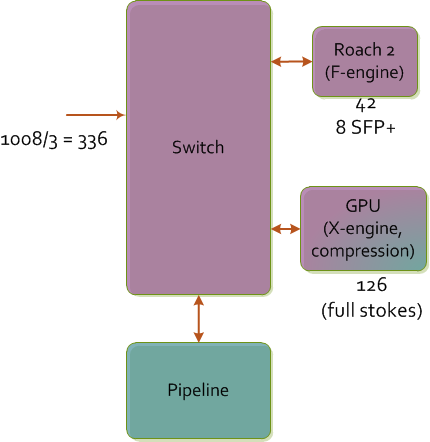
\includegraphics[width=0.55\textwidth]{plots/Digital.png}
\caption{Digital configuration.}
\label{fig:digital}
\end{figure}

The Roach 2 boards will serve as the F-engine for the correlator.  Each will
have 8 bi-directional (?) SFP+ connectors.  Since at this point there are still
3 antennas per link, there are 1008/3/8 = 42 Roach 2 boards.

The GPUs will serve as the X-engine (and compression, as discussed below).  It
is anticipated that in the timeframe of the proposal, a GPU box containing 1
CPU and 2 GPUs will handle 16 ant-pols at full Stokes.  For the 1008 $\times$ 2
= 2016 ant-pols, that is then 126 boxes.  Note that full Stokes is likely not
needed, and the GPU system may possibly be reduced.

The switch will need 336 + 42 + 126 = 504 inputs.  How does data get to
storage???

\section{Processing}

As noted above, about 3.3 Tbps is streaming through the correlator, which is
too much to fully archive.  A near-real-time pipelined processing system must
therefore be in place to handle the data and save an appropriate data volume.

Details of the processing/compression, leading to the use of the GPUs during the day to process.

\section{Infrastructure}
Need some.

\section{Costing}

The section provides a rough top-down costing of the proposed system.  It is
based on current known pricing with Moore's law applied as appropriate.  Tables
\ref{tab:costingElement} - \ref{tab:costingOverall} provide an overview of the
budget. 

%%%%%%%%%%%%%%%%%%%%%%TABLE:  ELEMENT
\begin{table}[h]
\begin{center}
\caption{\label{tab:costingElement}Top-down costing of strawman system:  \bf Element}
\begin{tabular}{ | p{2in} | c | c | r |}
\hline
\bf Description & \bf Each & \bf Number & \bf Total [k] \\
\hline
Ground screen & \$150 & 1008 & \$152 \\
\hline
Dipole & \$50 & 1008 & \$51 \\
\hline
Balun & \$250 & 1008 & \$252 \\
\hline
Cal load & \$50 & 1008 & \$51 \\
\hline
Cable (all cables, say 50ft at \$5/ft?) & \$250 & 1008 & \$252 \\
\hline
Labor & \$800 & 1008 & \$806 \\
\hline
\multicolumn{3}{| l |}{\bf Sub-total} & \$1564 \\
\hline
\end{tabular}
\end{center}
\end{table}

%%%%%%%%%%%%%%%%%%%%%%TABLE:  NODE
\begin{table}[h]
\begin{center}
\caption{\label{tab:costingNode}Top-down costing of strawman system:  \bf Node}
\begin{tabular}{ | p{2in} | c | c | r |}
\hline
\bf Description & \bf Each & \bf Number & \bf Total [k] \\
\hline
Phase switch & \$50 & 1008 & \$51 \\
\hline
Receiver & \$200 & 1008 & \$202 \\
\hline
Dual ADC & \$250 & 1008 & \$252 \\
\hline
2 x optical link & \$300 & 1008 & \$303 \\
\hline
MUX - how to handle this?  & \$300 & 1008 & \$303 \\
\hline
FPGA ???I have no idea & \$500 & 1008 & \$504 \\
\hline
10 GbE cable & \$100 & 1008 & \$101 \\
\hline
GPS & \$400 & 336 & \$135 \\
\hline
Clock ???& \$100 & 336 & \$34 \\
\hline
Sensors??? & \$50 & 336 & \$17 \\
\hline
Cooling/regulation??? & \$200 & 336 & \$68 \\
\hline
Packaging??? & \$100 & 336 & \$34 \\
\hline
Power & \$500 & 336 & \$168 \\
\hline
Labor & \$1000 & 336 & \$336 \\
\hline
\multicolumn{3}{| l |}{\bf Sub-total} & \$2508 \\
\hline
\end{tabular}
\end{center}
\end{table}

%%%%%%%%%%%%%%%%%%%%%%TABLE:  DIGITAL
\begin{table}[h]
\begin{center}
\caption{\label{tab:costingDigital}Top-down costing of strawman system:  \bf Digital}
\begin{tabular}{ | p{2in} | c | c | r |}
\hline
\bf Description & \bf Each & \bf Number & \bf Total [k] \\
\hline
Switch & \$500 & 504 & \$252 \\
\hline
Roach 2 & \$6000 & 42 & \$252 \\
\hline
GPU & \$7000 & 126 & \$882 \\
\hline
10 GbE Cable (8$\times$42+126+336=806) & \$100 & 806 & \$81 \\
\hline
Labor & \$100000 & 2 & \$200 \\
\hline
\multicolumn{3}{| l |}{\bf Sub-total} & \$1667 \\
\hline
\end{tabular}
\end{center}
\end{table}

%%%%%%%%%%%%%%%%%%%%%%TABLE:  COMPUTING
\begin{table}[h]
\begin{center}
\caption{\label{tab:costingCompute}Top-down costing of strawman system:  \bf{Computing/Archive}}
\begin{tabular}{ | p{2in} | c | c | r |}
\hline
\bf Description & \bf Each & \bf Number & \bf Total [k] \\
\hline
A & \$ &  & \$ \\
\hline
B 2 & \$ &  & \$ \\
\hline
C & \$ &  & \$ \\
\hline
D & \$ &  & \$ \\
\hline
Labor & \$ &  & \$ \\
\hline
\multicolumn{3}{| l |}{\bf Sub-total} & \$xx \\
\hline
\end{tabular}
\end{center}
\end{table}

%%%%%%%%%%%%%%%%%%%%%%TABLE:  INFRASTRUCTURE
\begin{table}[h]
\begin{center}
\caption{\label{tab:costingInfrastructure}Top-down costing of strawman system:  \bf{Infrastructure}}
\begin{tabular}{ | p{2in} | c | c | r |}
\hline
\bf Description & \bf Each & \bf Number & \bf Total [k] \\
\hline
Switch & \$ & 1 & \$500 \\
\hline
Labor & \$ &  & \$ \\
\hline
\multicolumn{3}{| l |}{\bf Sub-total} & \$500 \\
\hline
\end{tabular}
\end{center}
\end{table}

%%%%%%%%%%%%%%%%%%%%%%TABLE:  OVERALL
\begin{table}[h]
\begin{center}
\caption{\label{tab:costingOverall}Top-down costing of strawman system:  \bf{Overall}}
\begin{tabular}{| l | r |}
\hline
\bf Sub-system & \bf {Total [k]} \\
\hline
Element & \$1564 \\
\hline
Node & \$2508 \\
\hline
Digital & \$1667 \\
\hline
Computing & \$ \\
\hline
Infrastructure & \$500 \\
\hline
Labor & \$ \\
\hline
\bf{Grand Total} & \$6239 \\
\hline
\end{tabular}
\end{center}
\end{table}

\end{document}
